
\subsection{Attachment}
\label{sec:Attachment}

\begin{figure}[ht]
\begin{center}
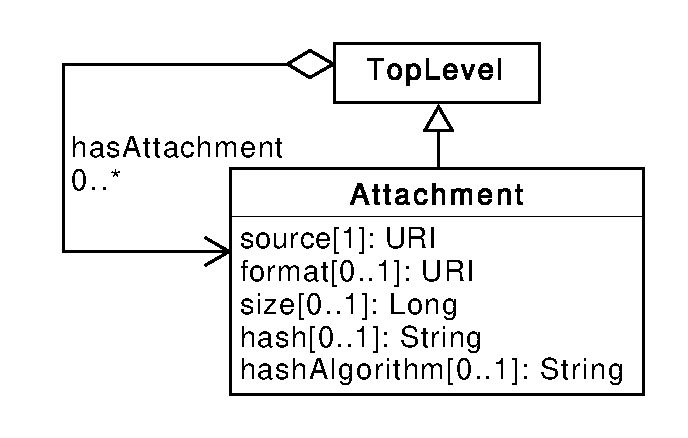
\includegraphics[scale=0.6]{uml/attachment}
\caption[]{Diagram of the \sbol{Attachment} class and its associated properties.}
\label{uml:attachment}
\end{center}
\end{figure}

The purpose of the \sbol{Attachment} class is to serve as a general container for data files, especially experimental data files.
It provides a means for linking files and metadata to SBOL designs.

The meta-data provided by the \sbol{Attachment} class include the following properties: the \sbolmult{source:A}{source} or location of the actual file of the attachment, the \sbol{format} of the file, the \sbol{size} of the file, and the \sbol{hash} for the file.

\subparagraph{ The \sbolheading{source} property}\label{sec:source:A}
The \sbolmult{source:A}{source} property is REQUIRED and MUST contain a \sbol{URI} reference to the source file.

\subparagraph{ The \sbolheading{format} property}\label{sec:format}
The \sbol{format} property is OPTIONAL and MAY contain a \sbol{URI} that specifies the format of the attached file. It is RECOMMENDED that this \sbol{URI} refer to a term from the EMBRACE Data and Methods (EDAM) ontology.

\subparagraph{ The \sbolheading{size} property}\label{sec:size}
The \sbol{size} property is OPTIONAL and MAY contain a long indicating the file size in bytes.

\subparagraph{ The \sbolheading{hash} property}\label{sec:hash}
The \sbol{hash} property is OPTIONAL and MAY contain a SHA-1 hash of the file contents represented as a hexadecimal digest.
